% Created 2024-02-18 Sun 13:41
% Intended LaTeX compiler: xelatex
\documentclass[11pt]{article}
\usepackage{hyperref}

%% ox-latex features:
%   !announce-start, !guess-pollyglossia, !guess-babel, !guess-inputenc, caption,
%   image, !announce-end.

\usepackage{capt-of}

\usepackage{graphicx}

%% end ox-latex features


\author{Guy E. Blelloch, Laxman Dhulipala, Yihan Sun}
\date{\today}
\title{Introduction to Parallel Algorithms}
\hypersetup{
 pdfauthor={Guy E. Blelloch, Laxman Dhulipala, Yihan Sun},
 pdftitle={Introduction to Parallel Algorithms},
 pdfkeywords={},
 pdfsubject={},
 pdfcreator={Emacs 30.0.50 (Org mode 9.7-pre)}, 
 pdflang={English}}
\begin{document}

\maketitle
\tableofcontents

% TIPS
% \substack{a\\b} for multiple lines text





% pdfplots will load xolor automatically without option
\usepackage[dvipsnames]{xcolor}

\usepackage{forest}
% two-line text in node by [two \\ lines]
% \begin{forest} qtree, [..] \end{forest}
\forestset{
  qtree/.style={
    baseline,
    for tree={
      parent anchor=south,
      child anchor=north,
      align=center,
      inner sep=1pt,
    }}}
%\usepackage{flexisym}
% load order of mathtools and mathabx, otherwise conflict overbrace

\usepackage{mathtools}
%\usepackage{fourier}
\usepackage{pgfplots}
\usepackage{amsthm, mathabx,  amsmath, commath}
\usepackage{amsfonts}

\usepackage{empheq}
\usepackage{tikz}
\usetikzlibrary{arrows.meta}
\usepackage[most]{tcolorbox}

\newtheorem{theorem}{Theorem}[section]
\newtheorem{definition}{Definition}[section]
\newtheorem{corollary}{Corollary}[section]
\newtheorem{example}{Example}[section]
\newtheorem{lemma}{Lemma}[section]
\newtheorem{proposition}{Proposition}[section]

\newcommand{\bl}[1] {\boldsymbol{#1}}
\newcommand{\Wt}[1] {\stackrel{\sim}{\smash{#1}\rule{0pt}{1.1ex}}}
\newcommand{\wt}[1] {\widetilde{#1}}


%For boxed texts in align, use Aboxed{}
%otherwise use boxed{}

\DeclareMathSymbol{\widehatsym}{\mathord}{largesymbols}{"62}
\newcommand\lowerwidehatsym{%
  \text{\smash{\raisebox{-1.3ex}{%
    $\widehatsym$}}}}
\newcommand\fixwidehat[1]{%
  \mathchoice
    {\accentset{\displaystyle\lowerwidehatsym}{#1}}
    {\accentset{\textstyle\lowerwidehatsym}{#1}}
    {\accentset{\scriptstyle\lowerwidehatsym}{#1}}
    {\accentset{\scriptscriptstyle\lowerwidehatsym}{#1}}
}

\usepackage{graphicx}
    
% text on arrow for xRightarrow
\makeatletter
%\newcommand{\xRightarrow}[2][]{\ext@arrow 0359\Rightarrowfill@{#1}{#2}}
\makeatother


\def \bx {\boldsymbol{x}}
\def \ba {\boldsymbol{a}}
\def \bI {\boldsymbol{I}}
\def \bt {\boldsymbol{t}}
\def \bb {\boldsymbol{b}}
\def \bA {\boldsymbol{A}}
\def \bX {\boldsymbol{X}}
\def \bu {\boldsymbol{u}}
\def \bS {\boldsymbol{S}}
\def \bZ {\boldsymbol{Z}}
\def \bz {\boldsymbol{z}}
\def \by {\boldsymbol{y}}
\def \bw {\boldsymbol{w}}
\def \bT {\boldsymbol{T}}
\def \bS {\boldsymbol{S}}
\def \bm {\boldsymbol{m}}
\def \bW {\boldsymbol{W}}
\def \bY {\boldsymbol{Y}}
\def \bH {\boldsymbol{H}}
\def \blambda {\boldsymbol{\lambda}}
\def \bPhi {\boldsymbol{\Phi}}
\def \btheta {\boldsymbol{\theta}}
\def \bmu {\boldsymbol{\mu}}
\def \bphi {\boldsymbol{\phi}}
\def \bSigma {\boldsymbol{\Sigma}}
\def \lb {\left\{}
\def \rb {\right\}}
\def \caln {\mathcal{N}}
\def \dissum {\displaystyle\Sigma}
\def \dispro {\displaystyle\prod}
\def \E {\mathbb{E}}
\def \Q {\mathbb{Q}}
\def \V {\mathbb{V}}
\def \R {\mathbb{R}}
\def \calq {\mathcal{Q}}
\def \calg {\mathcal{G}}
\def \caln {\mathcal{N}}
\def \calr {\mathcal{R}}
\def \calm {\mathcal{M}}
\def \calc {\mathcal{C}}
\def \bcup {\bigcup}

\graphicspath{{../../books/}}
\algrenewcommand\algorithmicforall{\textbf{parfor}}

From \url{https://www.cs.cmu.edu/\~guyb/paralg/paralg/parallel.pdf}
\section{Models}
\label{sec:org49fb2bb}
We use the \textbf{Random Access Machine} (RAM) model which consists of a single processor with some constant
number of registers, an instruction counter and an arbitrarily large memory. The RAM model assumes
that all instructions take unit time.

The RAM is by no stretch meant to model the runtime on a real machine with cycle-by-cycle level
accuracy. It does not model, for example, that modern-day machines have cache hierarchies and
therefore not all memory accesses are equally expensive.

In \textbf{work-span} models, algorithms still assume a shared random access memory, but allow dynamically
creating tasks. Costs are measured in terms of the total number of operations, the \textbf{work} and the
longest chain of dependence.

We call a parallel algorithm \textbf{work-efficient} if its work is work asymptotically the same as its
best-known sequential counterpart.

The span for a parallel algorithm is the running time when you have an infinite number of processors.

The \textbf{Multi-Process Random-Access Machine} (MP-RAM) consists of a set of processes that share an
unbounded memory. The MP-RAM extends the RAM with a fork instruction that takes a positive integer
\(k\) and forks \(k\) new child processes. Each child process receives a unique integer in the range
\([1, . . . , k]\) in its first register and otherwise has the identical state as the parent (forking
process), which has that register set to 0. All children start by running the next instruction, and
the parent suspends until all the children terminate (execute an end instruction). The first
instruction of the parent after all children terminate is called the \textbf{join} instruction. A \textbf{computation}
starts with a single root process and finishes when that root process ends. This model supports
\textbf{nested parallelism} -the ability to fork processes in a nested fashion. If the root process never does
a fork, it is a standard sequential program.

A computation in the MP-RAM defines a partial order on the instructions. In particular
\begin{enumerate}
\item every instruction depends on its previous instruction in the same thread (if any),
\item every first instruction in a process depends on the fork instruction of the parent that generated
it, and
\item every join instruction depends on the end instruction of all child processes of the corresponding
fork generated.
\end{enumerate}

The work of a computation is the total number of instructions, and the span is the longest sequences
of dependent instructions.

Two instructions are said to be \textbf{concurrent} if they are unordered, and ordered otherwise. Two
instructions \textbf{conflict} if one writes to a memory location that the other reads or writes the same
location. We say two instructions race if they are concurrent and conflict.

A \(\textsc{testAndSet}(x)\) (TS) instruction takes a reference to a memory location \(x\), checks if
the value of \(x\) is \texttt{false} and if so atomically sets it to \texttt{true} and returns \texttt{true}; if already \texttt{true} it
returns \texttt{false}.

A \(\textsc{compareAndSwap}(x, o, n)\) (CAS) instruction takes a reference to a memory location \(x\),
checks if the value of \(x\) equals \(o\). If so, the instruction will change the value to \(n\) and
return \texttt{true}. If not, the instruction does nothing and simply returns \texttt{false}.

A \(\textsc{fetchAndAdd}(x, y)\) (FA) instruction takes a reference to a memory location \(x\), and a
value \(y\), and it adds \(y\) to the value of \(x\), returning the old value. Different from a TS or
a CAS, an FA instruction always successfully adds \(y\) to the value stored in \(x\).

A \(\textsc{priorityWrite}(x, y)\) (PW) instruction takes a reference to a memory location \(x\), and
checks if the value \(y\) is less than the current value in \(x\). If so, it changes the value stored
in \(x\) to \(y\), and return \texttt{true}. If not, it does nothing and return \texttt{false}.
\section{Preliminaries}
\label{sec:org997ce75}
\begin{definition}[w.h.p.]
\(g(n)\in O(f(n))\) with \textbf{high probability} (w.h.p.) if \(g(n)\in O(cf(n))\) with probability at least
\(1-(\frac{1}{n})^c\), for some constant \(c_0\) and all \(c\ge c_0\).
\end{definition}

\begin{theorem}[]
Consider a set of indicator random variables \(X_1,\dots,X_n\) for which \(p(X_i=1)\le\barp_i\) conditioned on
all possible events \(X_j=\{0,1\}\), \(i\neq j\). Let \(X=\sum_{i=1}^nX_i\) and \(\barE[X]=\sum_{i=1}^n\barp_i\),
then
\begin{equation*}
\Pr[X\ge k]\le\left( \frac{e\barE[X]}{k} \right)^k
\end{equation*}
\end{theorem}

\begin{proof}
Let's first consider the special case that the \(\barp_i\) are all equal and have value \(p\). If
\(X\ge k\), then we have that at least \(k\) of the random variables are 1. The probability of any
particular \(k\) variables all being 1, and the others being anything, is upper bounded by \(p^k\).
\begin{equation*}
\Pr[X\ge k]\le p^k\binom{n}{k}<p^k\left(\frac{ne}{k}\right)^k
=\left(\frac{pne}{k}\right)^k=
\left(\frac{e\barE[X]}{k}\right)^k
\end{equation*}
Here we used a standard upper bound on the binomial coefficients: \(\binom{n}{m}<\left(\frac{ne}{m}\right)^m\).
\end{proof}
\section{Some Building Blocks}
\label{sec:orgb536966}
\subsection{Scan}
\label{sec:orge21bf3a}
A \textbf{scan} or \textbf{prefix-sum} function takes a sequence \(A\), an associative function \(f\), and a left
identity element \(\bot\) and computes the values
\begin{equation*}
r_i=
\begin{cases}
\bot&i=0\\
f(r_{i-1},A_i)&0<i\le\abs{A}
\end{cases}
\end{equation*}
Each \(r_i\) is the ``sum'' of the prefix \(A[0,i]\) of \(A\) w.r.t. the function \(f\).

\begin{algorithmic}
\Function{scanUp}{\(A,L,f\)}
\If{\(\abs{A}=1\)}
        \Return \(\abs{A[0]}\)
\Else
        \State \(n\gets\abs{A}\);
        \State \(m\gets n/2\);
        \State \(l\gets\textsc{scanUp}(A[0:m],L[0:m-1],f)\quad||\)
        \State \(r\gets\textsc{scanUp}([A[m:n],L[m:n-1]],f)\);
        \State \(L[m-1]\gets l\);
        \State \Return \(f(l,r)\)
\EndIf
\EndFunction
\end{algorithmic}

\begin{algorithmic}
\Function{scanDown}{\(R,L,f,s\)}
        \If{\(\abs{R}=1\)}
                \State \(R[0]=s\);
                \State \Return
        \Else
                \State \(n\gets\abs{A}\);
                \State \(m\gets\abs{R}/2\);
                \State \(\textsc{scanDown}(R[0:m],L[0:m-1],s)\quad||\)
                \State \(\textsc{scanDown}(R[m:n],L[m:n-1],f(s,L[m-1]))\);
                \State \Return
        \EndIf
\EndFunction
\end{algorithmic}

\begin{algorithmic}
\Function{scan}{\(A,f,I\)}
\State \(L\gets\textsc{array}[\abs{A}-1]\);
\State \(R\gets\textsc{array}[\abs{A}]\);
\State \(\texttt{total}\gets\textsc{scanUp}(A,L,f)\);
\State \(\textsc{scanDown}(R,L,f,I)\);
\State\Return \(\la R,\texttt{total}\ra\)
\EndFunction
\end{algorithmic}

For \textsc{scanUp} it should be clear that the values written into \(L\) are indeed the sums of the
left subtrees. For \textsc{scanDown} consider a node \(v\) in the tree and the value \(s\) passed to
it. The algorithm maintains that the value \(s\) is the sum of all values to the left of the subtree
rooted at \(v\).

\begin{center}
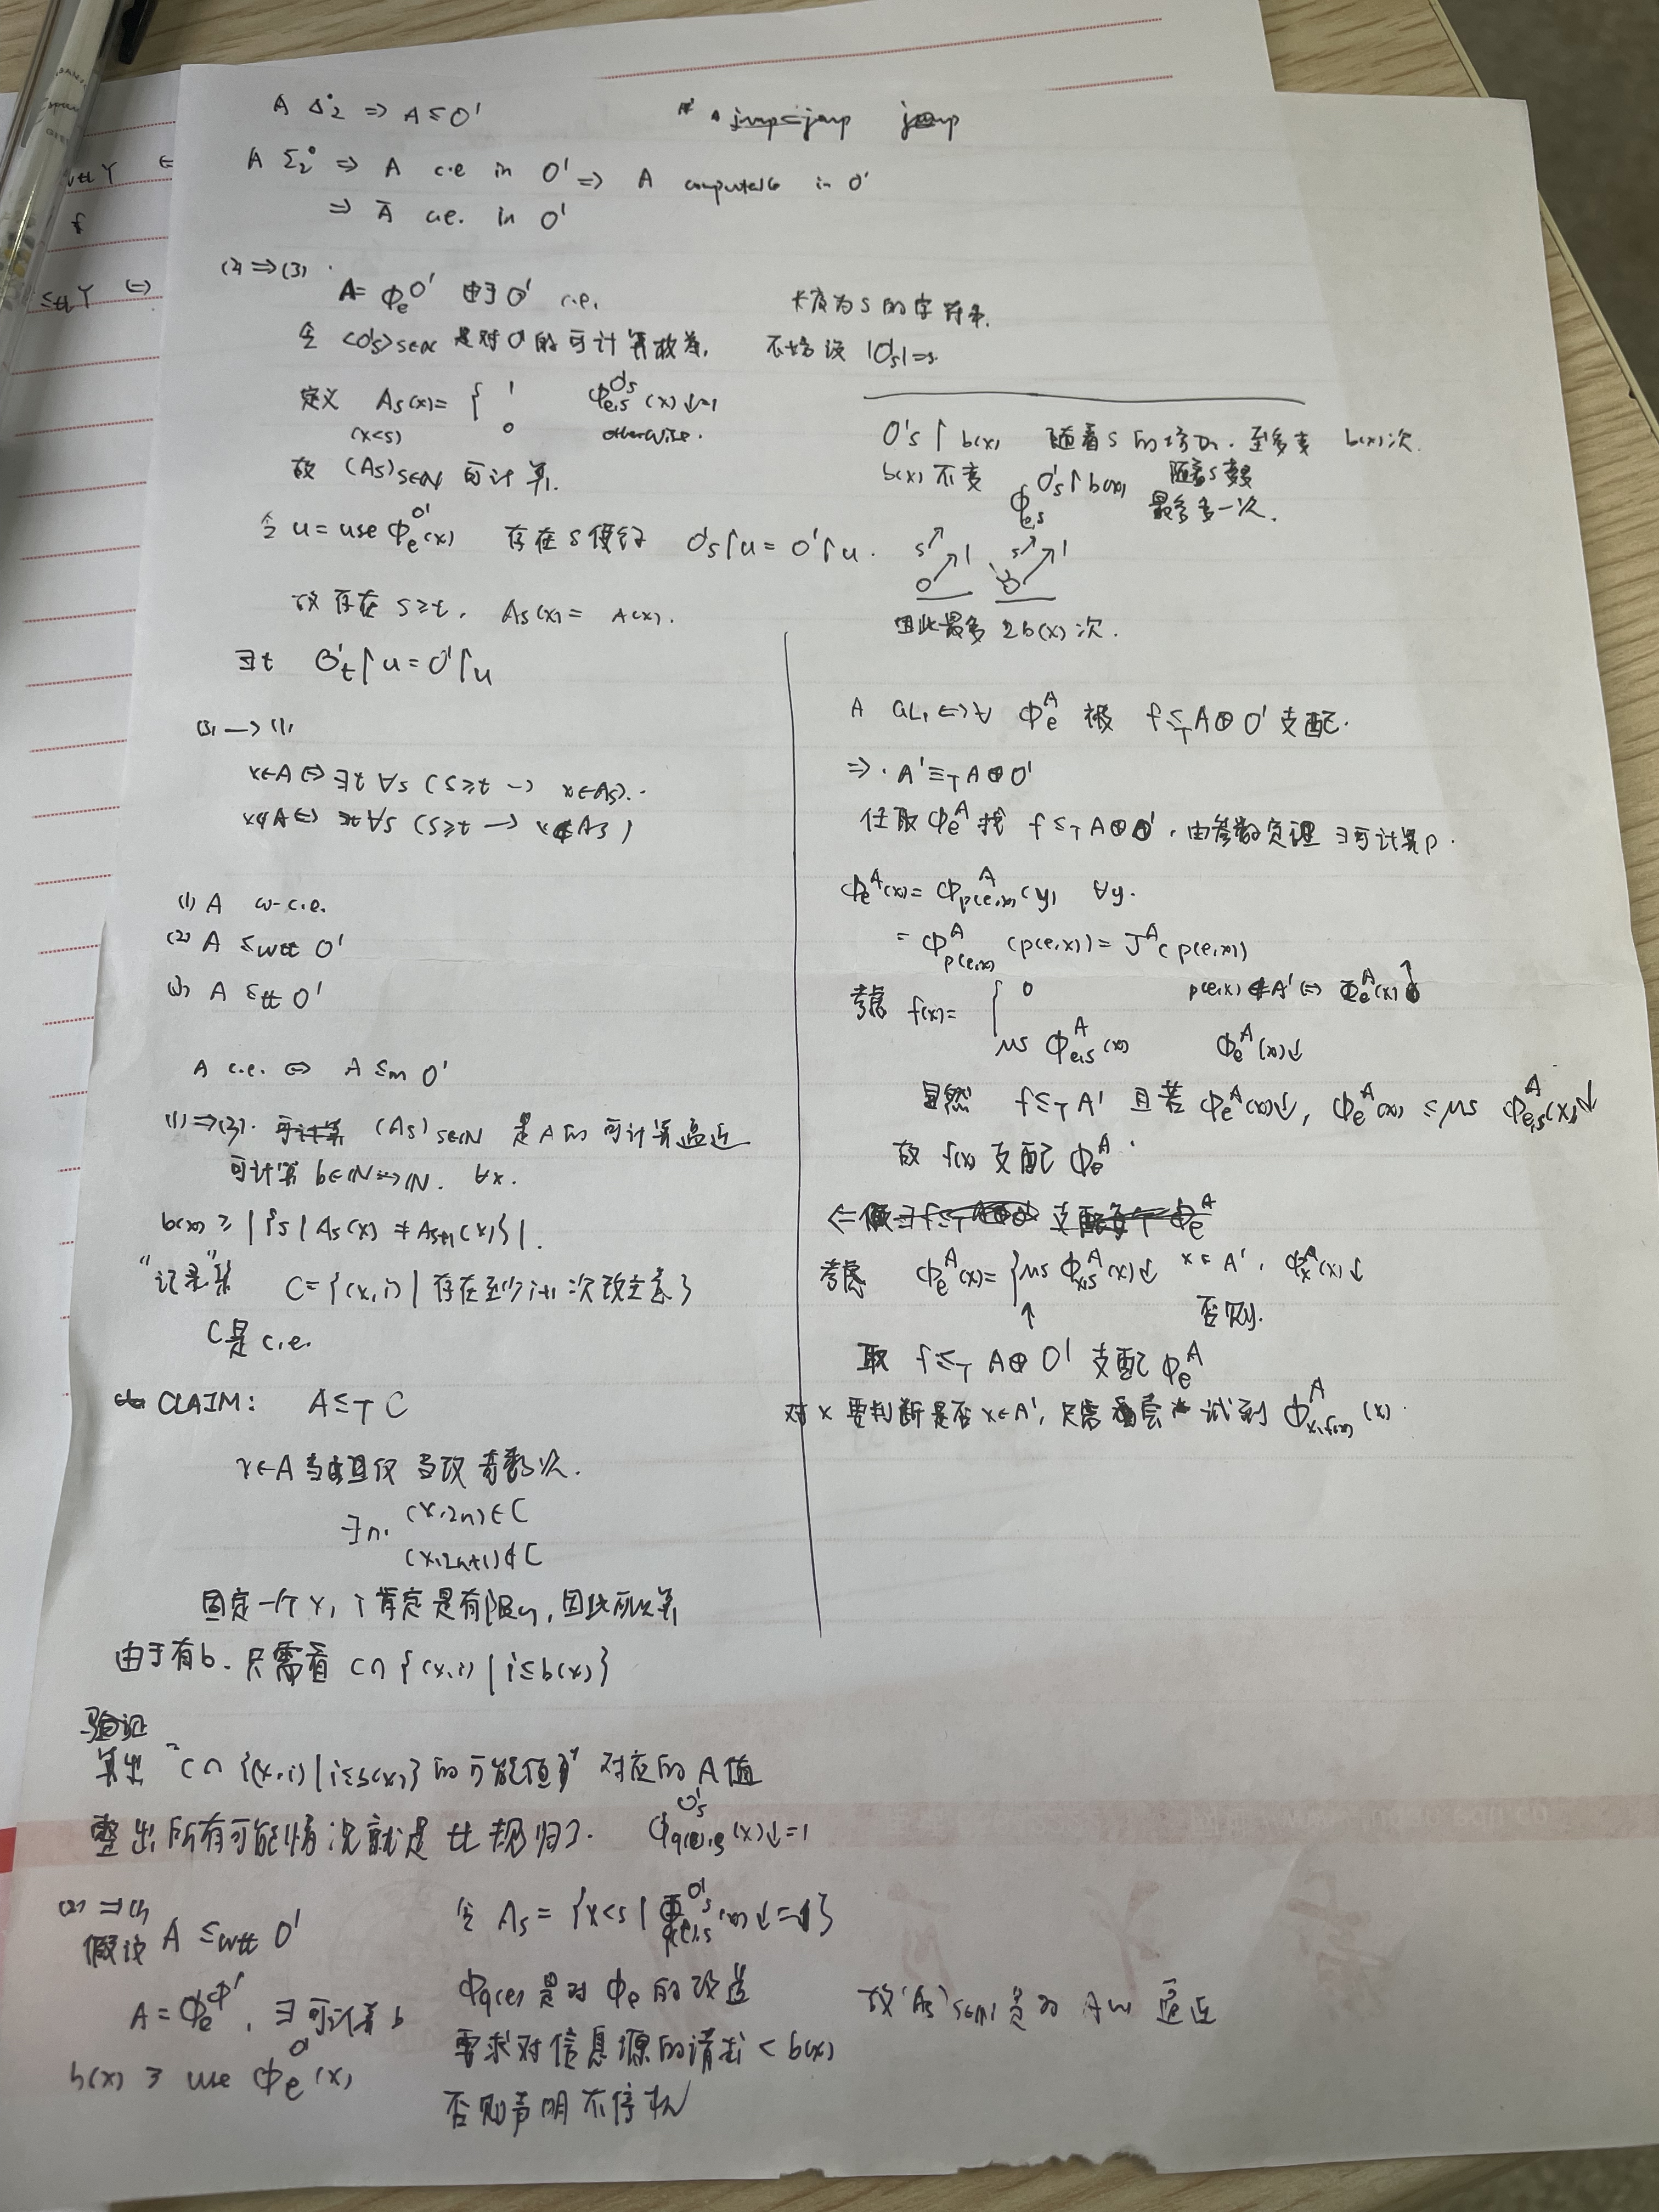
\includegraphics[width=.8\textwidth]{../images/Parallel/1.png}
\label{}
\end{center}
Work of \textsc{scanUp} and \textsc{scanDown} is
\begin{equation*}
W(n)=2W(n/2)+O(1)=O(n)
\end{equation*}
and the span is
\begin{equation*}
D(n)=D(n/2)+O(1)=\log(n)
\end{equation*}
\subsection{Filter and Flatten}
\label{sec:orga8d8650}
\begin{algorithmic}
\Function{filter}{\(A,p\)}
        \State \(n\gets\abs{A}\);
        \State \(F\gets\textsc{array}[n]\);
        \ForAll{\(i\in[0:n]\)}
        \State \(F[i]\gets p(A[i])\)
        \EndFor
        \State \(\la X,m\ra\gets\textsc{plusScan}(F)\);
        \State \(R\gets\textsc{array}[m]\);
        \ForAll{\(i\in[0:n]\)}
        \If{\(F[i]\)}
                \State\(R[X[i]]\gets A[i]\);
        \EndIf
        \EndFor
        \State\Return \(R\)
\EndFunction
\end{algorithmic}
\end{document}
